\begingroup
\let\clearpage\relax
\centerline{\textbf{APPENDIX}}
\vspace{0.5em}
%\chapter*{\textbf{APPENDIX}\linebreak Plots of potentiation over time}
\chapter*{Plots of potentiation over time}
\label{chap:app_a}
\endgroup

\begin{figure}[!h]
    \begin{center}
    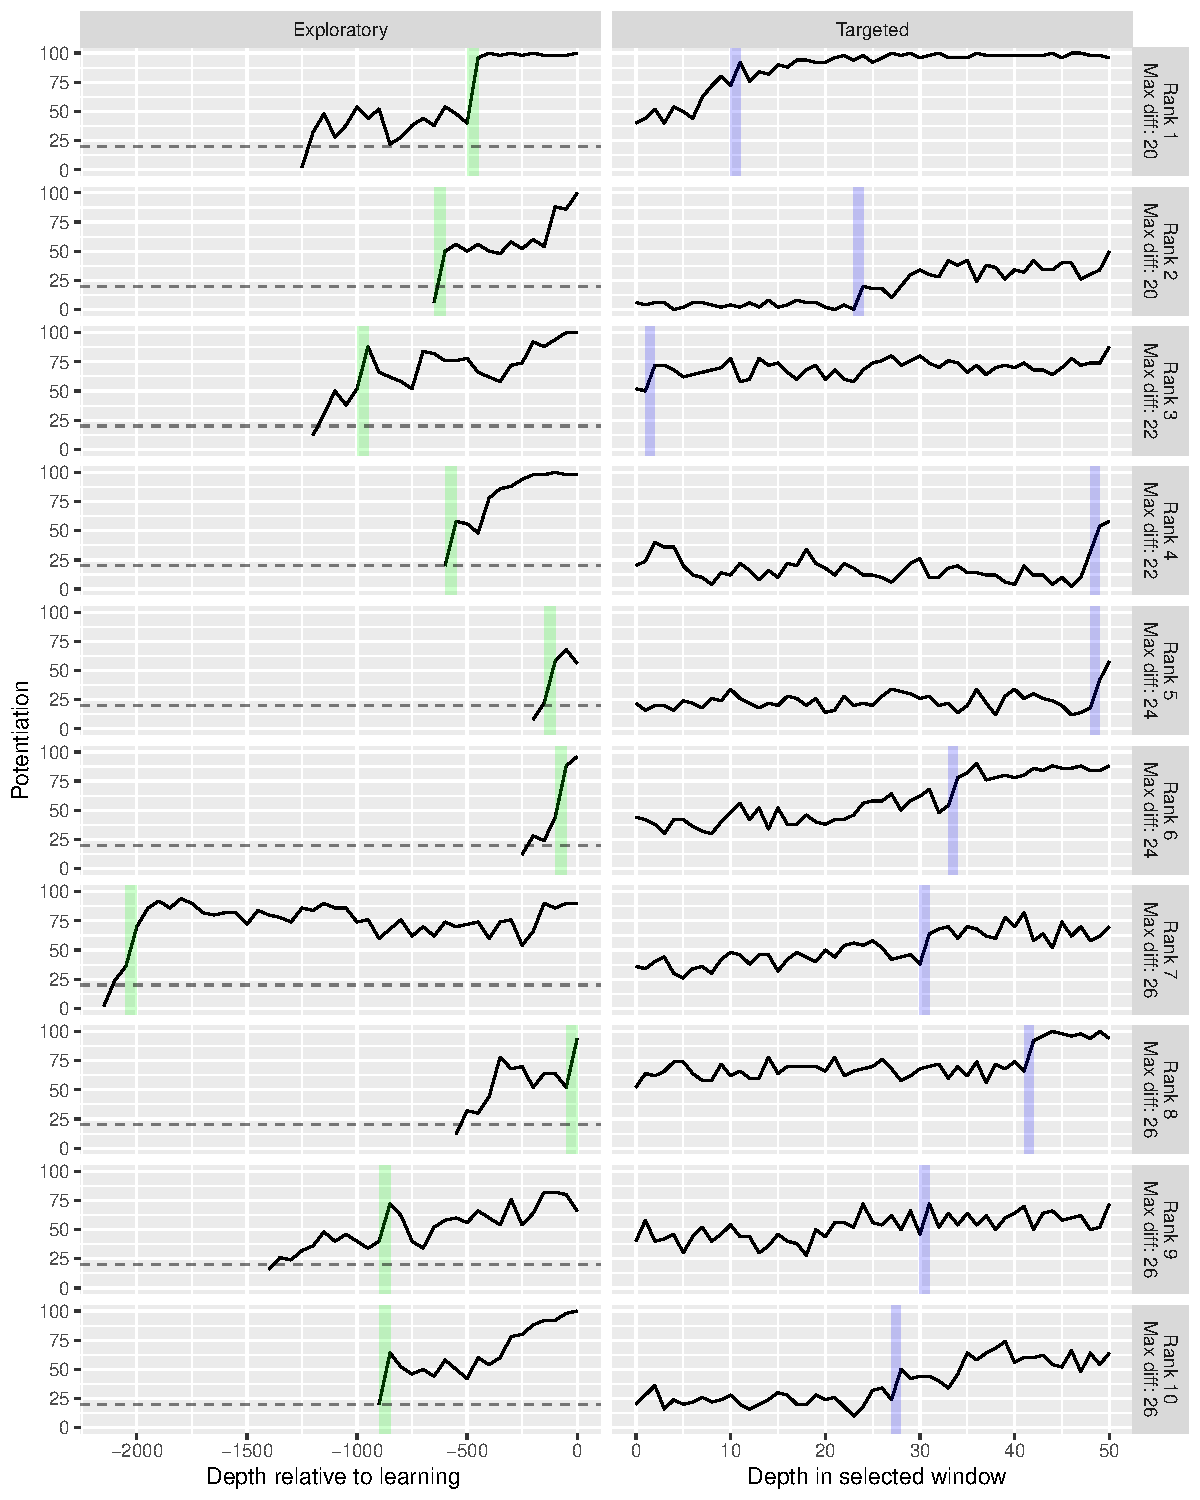
\includegraphics[width=0.85\textwidth]{07_appendix_potentiation_over_time/media/reps_1_10.pdf}
    \caption{Potentiation over time plots from Chapter \ref{chap:learning_distributions}.
    Left panes show exploratory replays, with a green rectangle indicating the 50-step window with the largest increase in potentiation. 
    Right panes show targeted replays, with the blue rectangle highlighting the largest single-step potentiation increase.
    Plots are ordered by the maximum single-step potentiation difference. }
    \label{fig:app_a_1_10}
    \end{center}
\end{figure}

\begin{figure}[!h]
    \begin{center}
    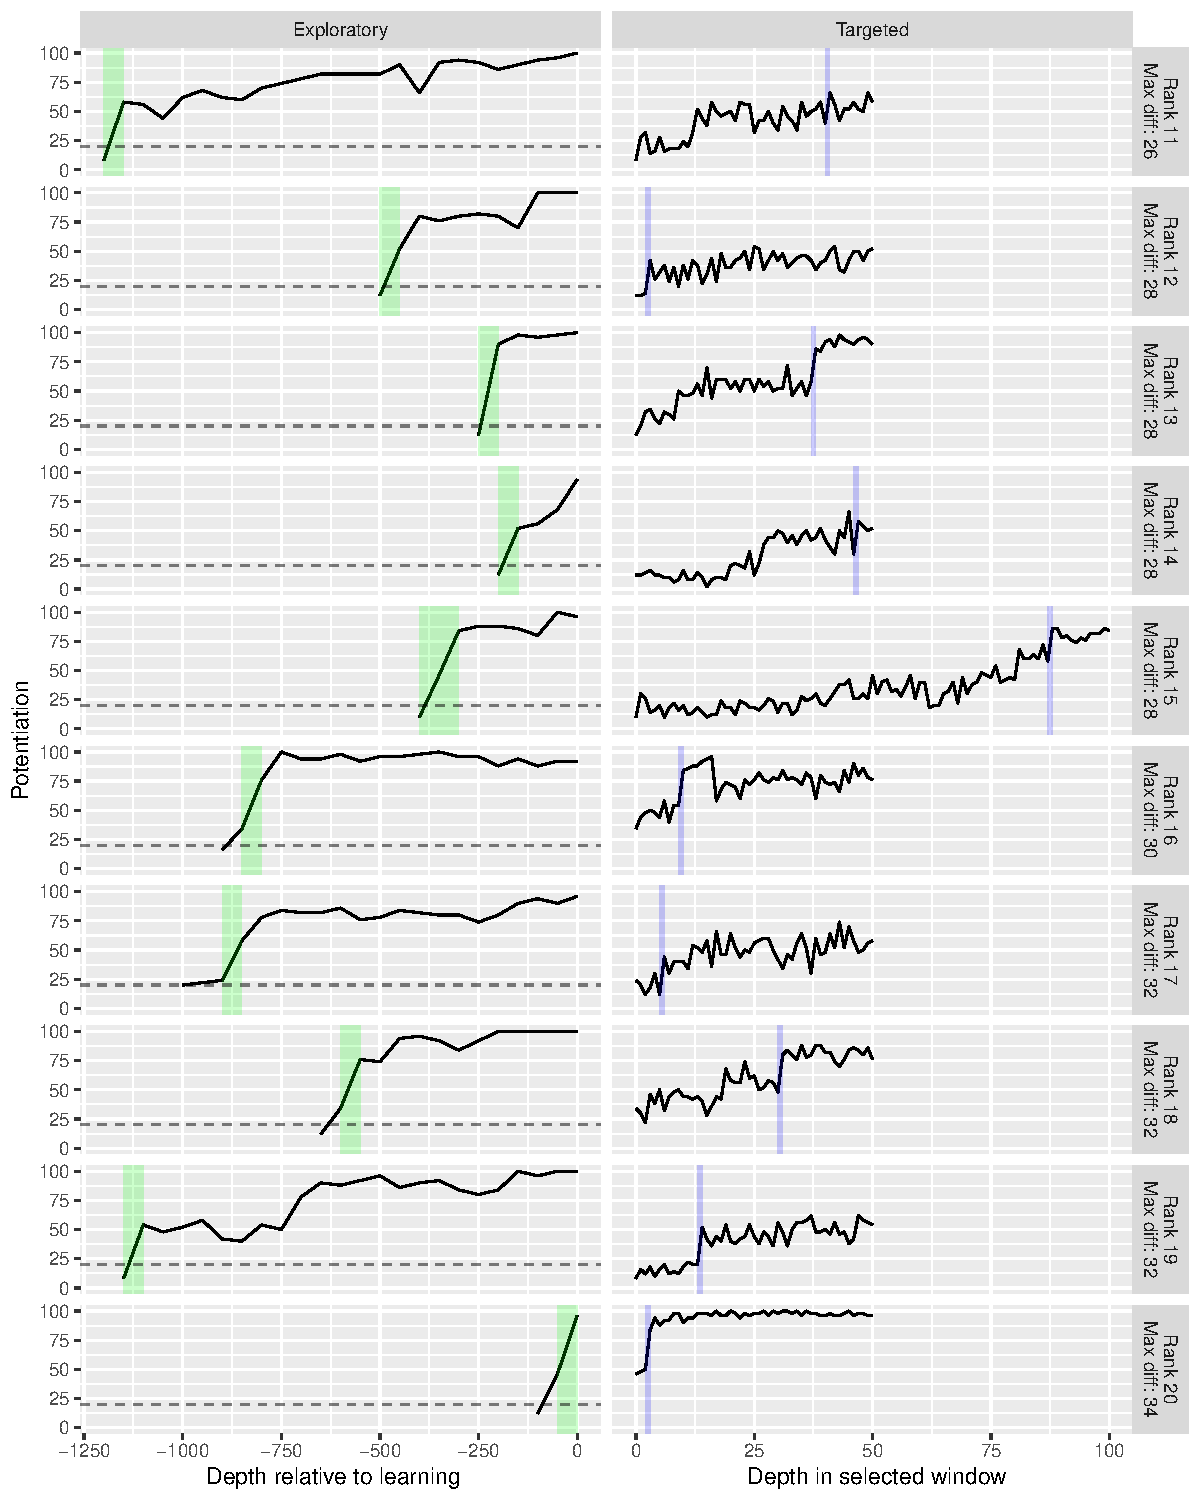
\includegraphics[width=0.9\textwidth]{07_appendix_potentiation_over_time/media/reps_11_20.pdf}
    \caption{Potentiation over time plots from Chapter \ref{chap:learning_distributions}.
    Left panes show exploratory replays, with a green rectangle indicating the 50-step window with the largest increase in potentiation. 
    Right panes show targeted replays, with the blue rectangle highlighting the largest single-step potentiation increase.
    Plots are ordered by the maximum single-step potentiation difference.}
    \label{fig:app_a_11_20}
    \end{center}
\end{figure}

\begin{figure}[!h]
    \begin{center}
    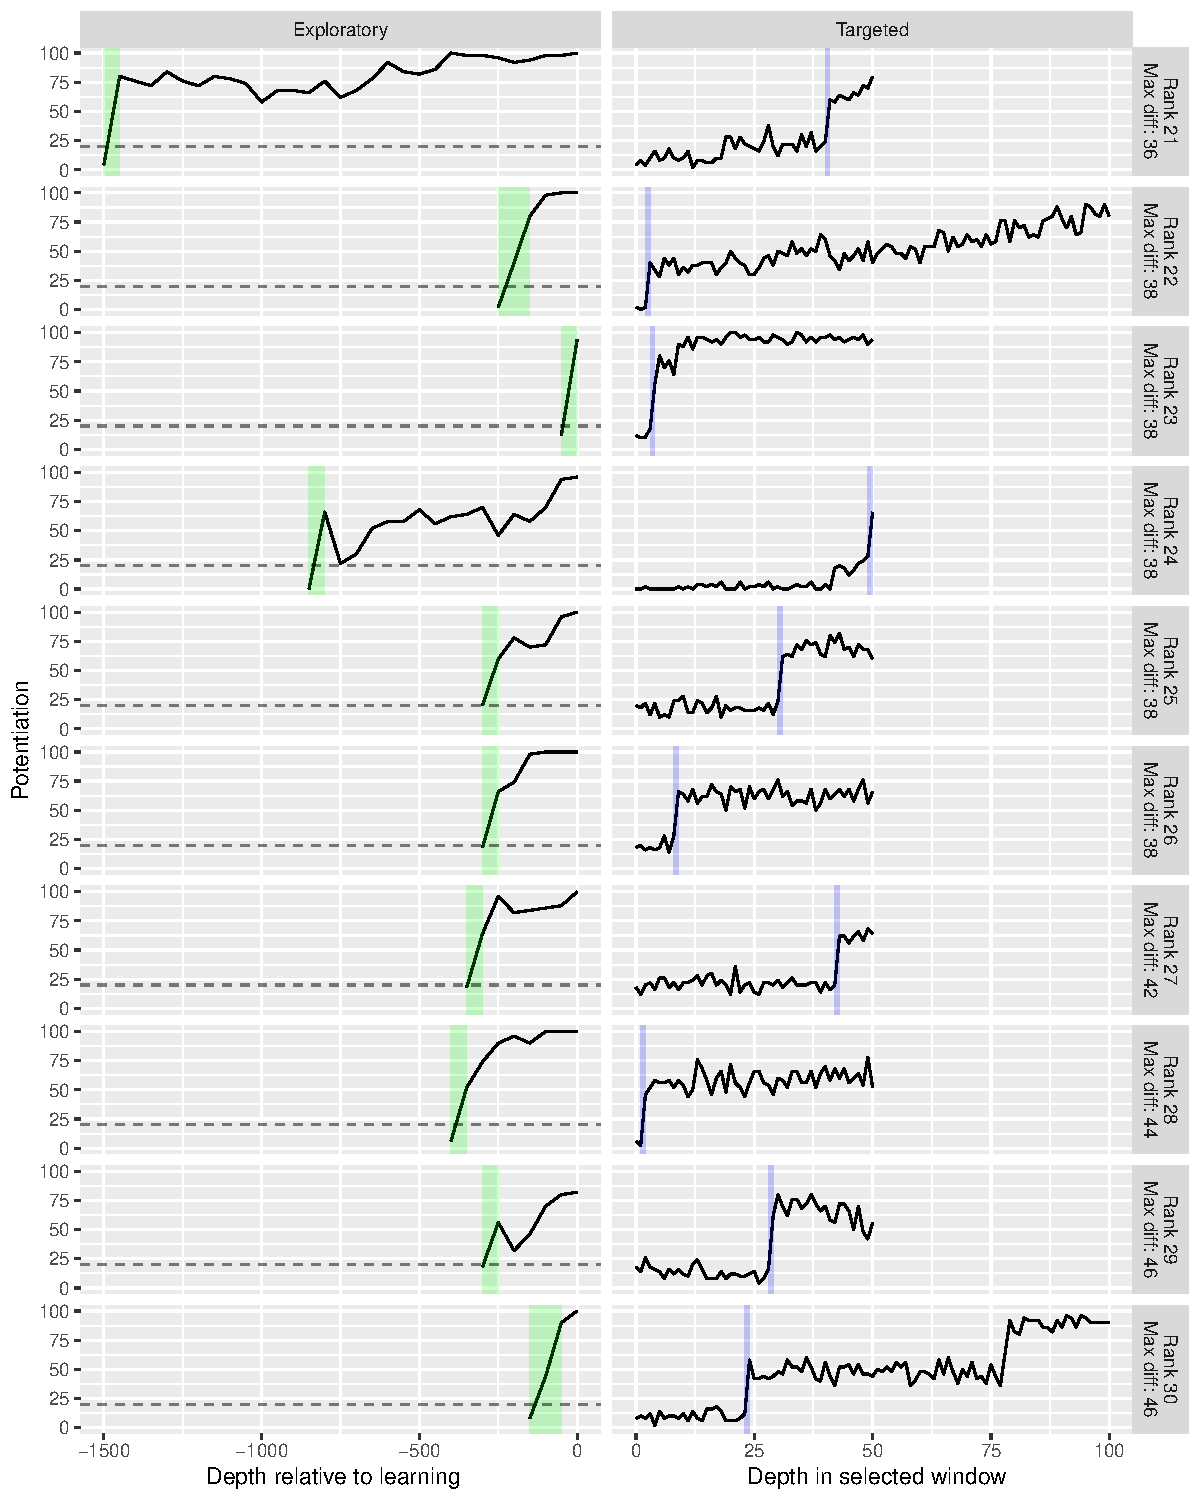
\includegraphics[width=0.9\textwidth]{07_appendix_potentiation_over_time/media/reps_21_30.pdf}
    \caption{Potentiation over time plots from Chapter \ref{chap:learning_distributions}.
    Left panes show exploratory replays, with a green rectangle indicating the 50-step window with the largest increase in potentiation. 
    Right panes show targeted replays, with the blue rectangle highlighting the largest single-step potentiation increase.
    Plots are ordered by the maximum single-step potentiation difference.}
    \label{fig:app_a_21_30}
    \end{center}
\end{figure}

\begin{figure}[!h]
    \begin{center}
    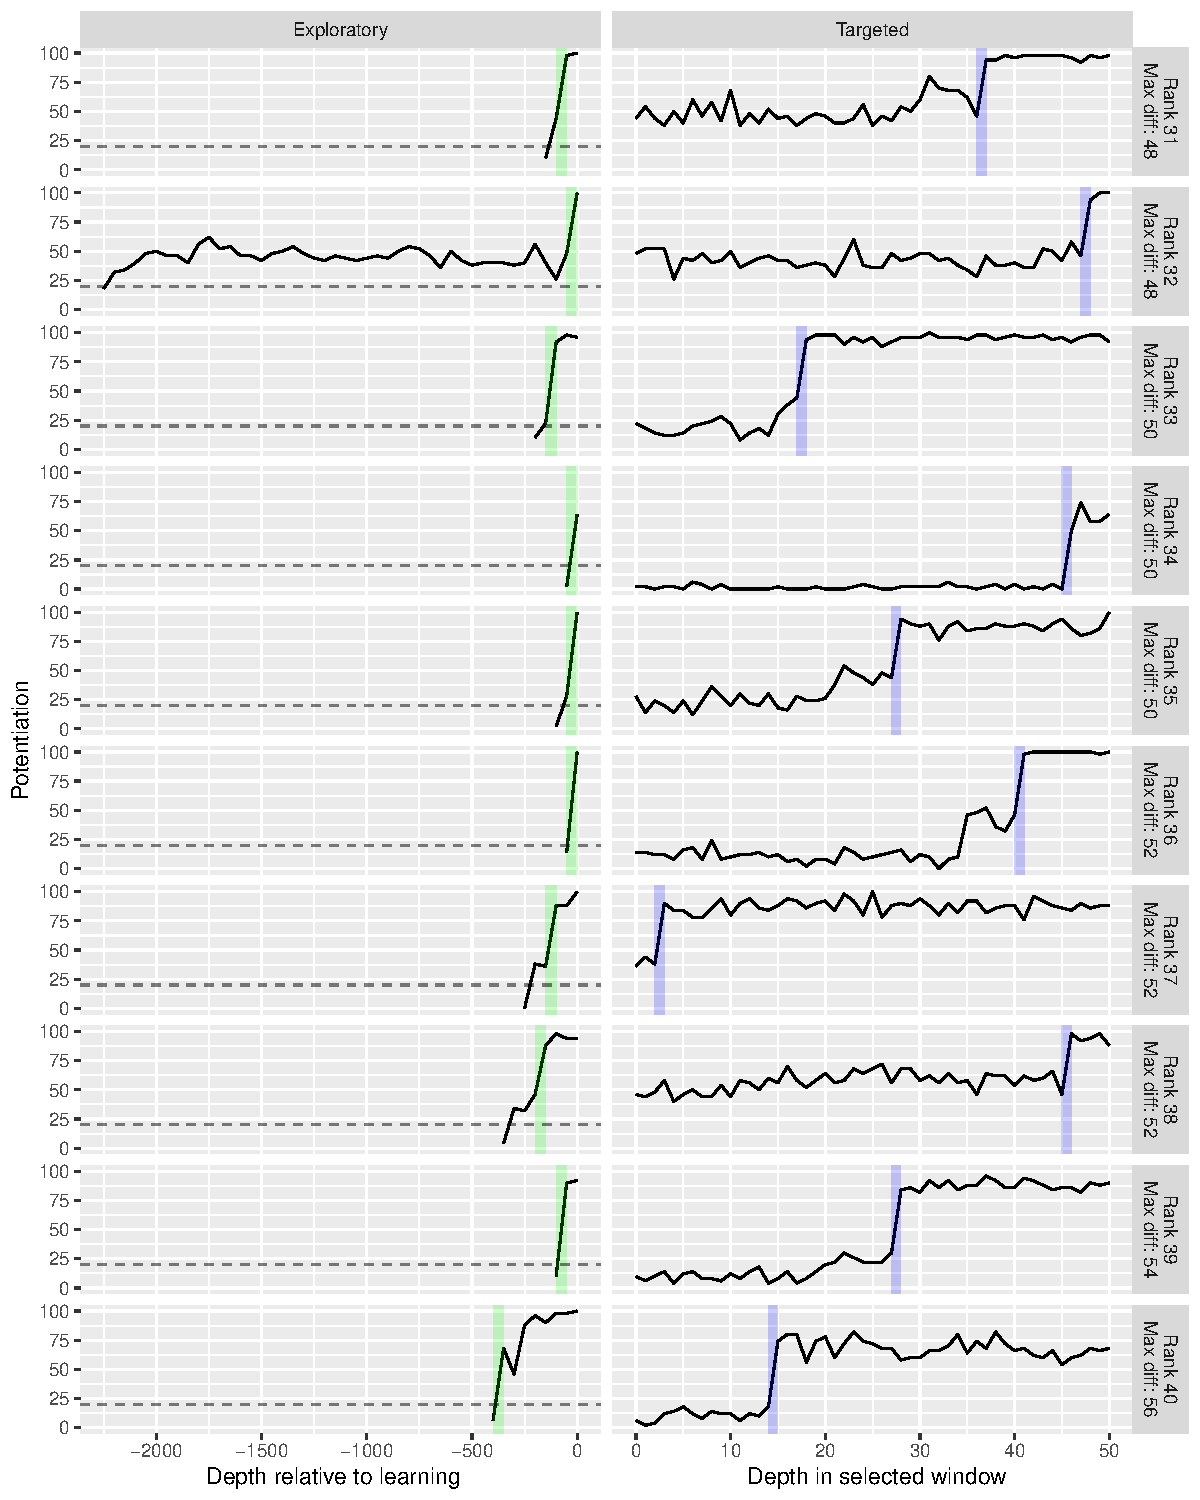
\includegraphics[width=0.9\textwidth]{07_appendix_potentiation_over_time/media/reps_31_40.pdf}
    \caption{Potentiation over time plots from Chapter \ref{chap:learning_distributions}.
    Left panes show exploratory replays, with a green rectangle indicating the 50-step window with the largest increase in potentiation. 
    Right panes show targeted replays, with the blue rectangle highlighting the largest single-step potentiation increase.
    Plots are ordered by the maximum single-step potentiation difference.}
    \label{fig:app_a_31_40}
    \end{center}
\end{figure}

\begin{figure}[!h]
    \begin{center}
    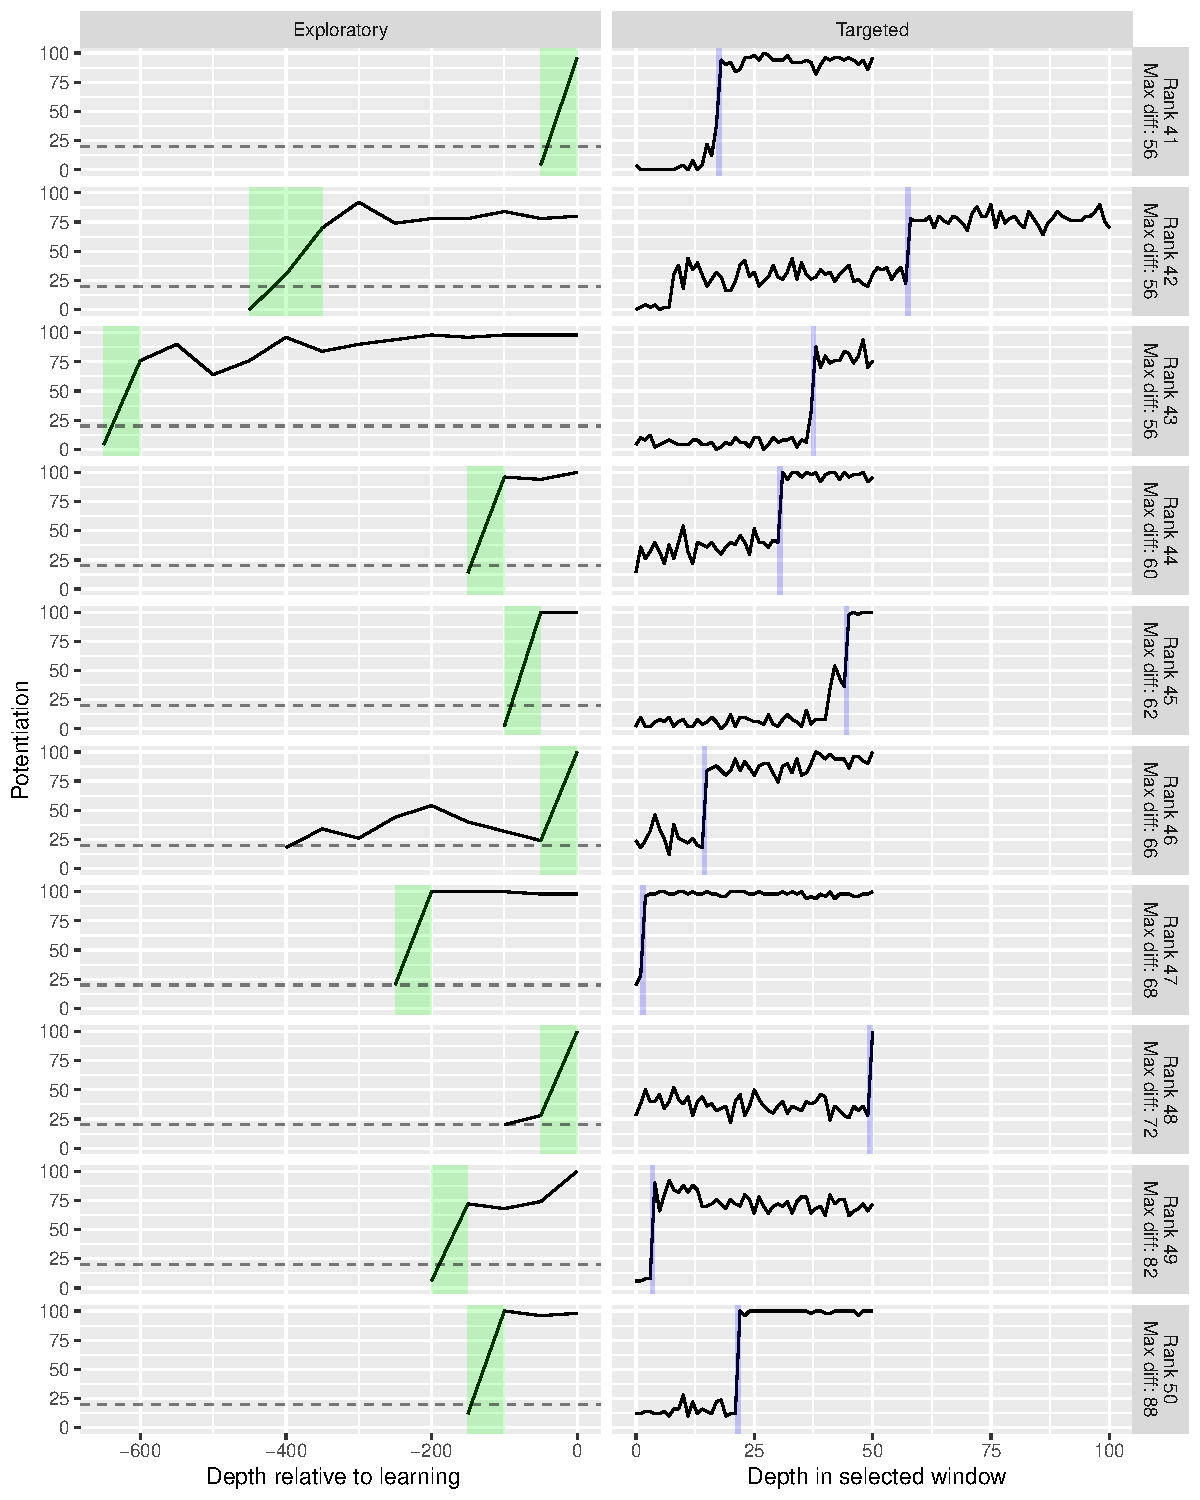
\includegraphics[width=0.9\textwidth]{07_appendix_potentiation_over_time/media/reps_41_50.pdf}
    \caption{Potentiation over time plots from Chapter \ref{chap:learning_distributions}.
    Left panes show exploratory replays, with a green rectangle indicating the 50-step window with the largest increase in potentiation. 
    Right panes show targeted replays, with the blue rectangle highlighting the largest single-step potentiation increase.
    Plots are ordered by the maximum single-step potentiation difference.}
    \label{fig:app_a_41_50}
    \end{center}
\end{figure}

\begin{figure}[!h]
    \begin{center}
    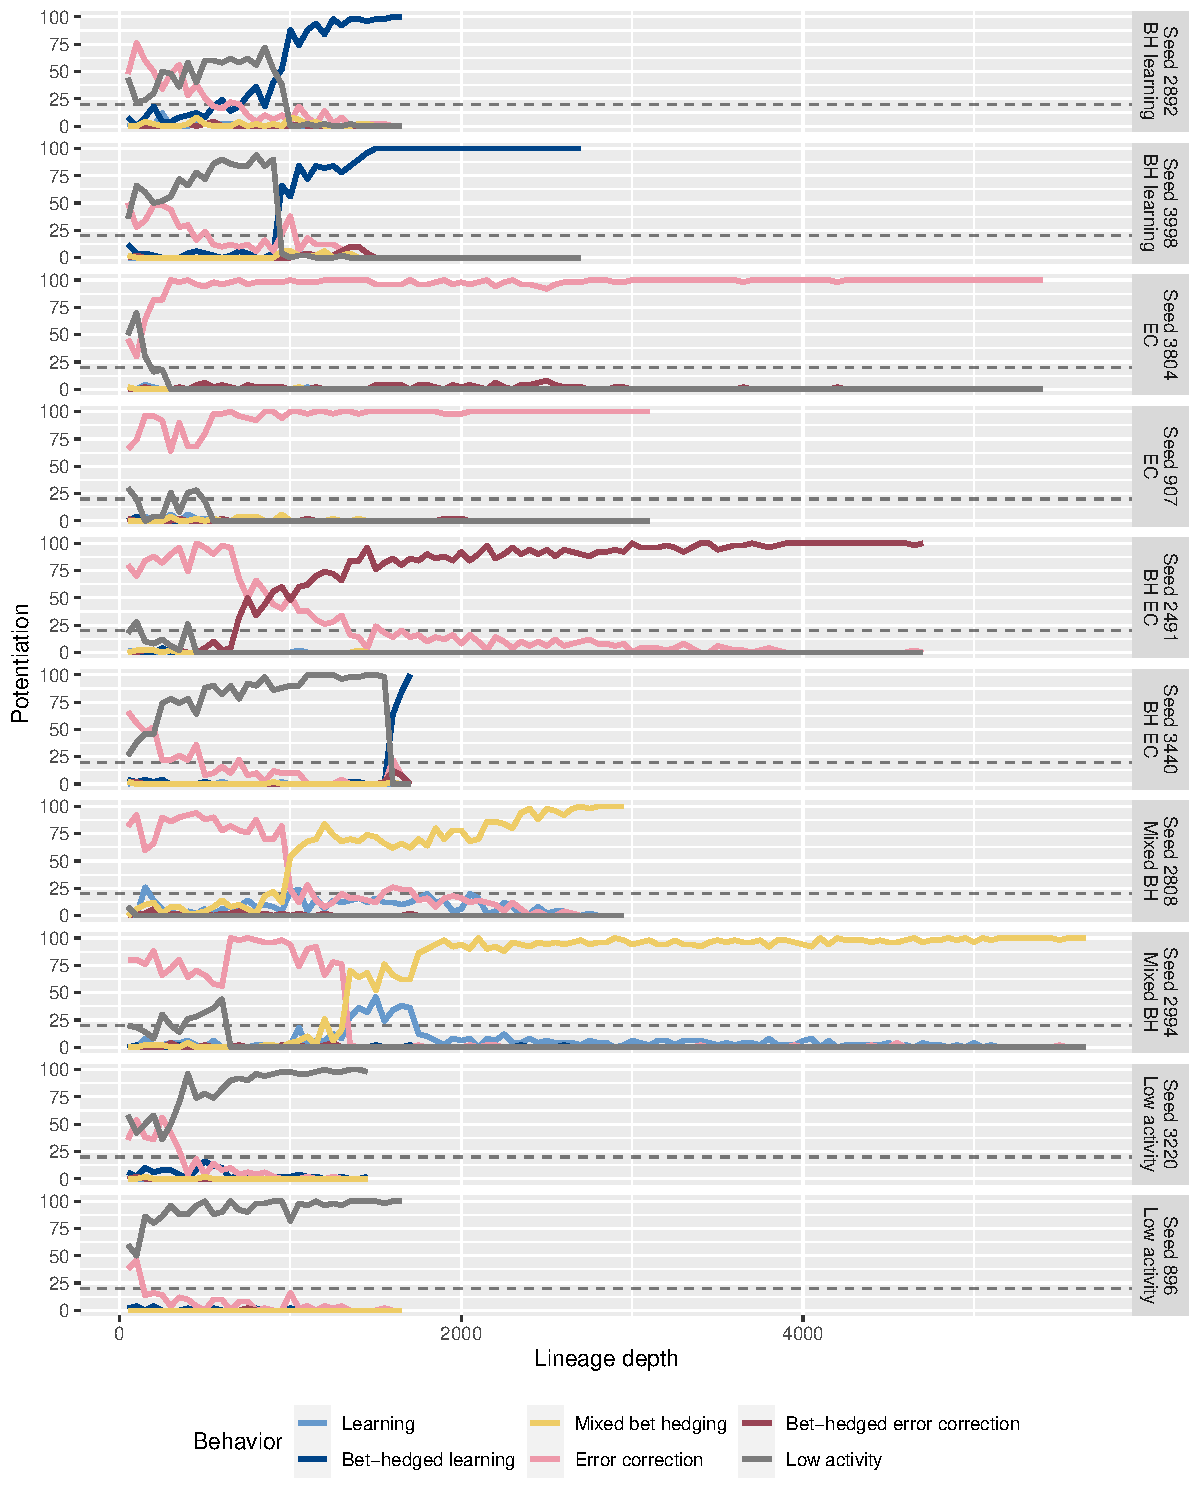
\includegraphics[width=0.9\textwidth]{07_appendix_potentiation_over_time/media/non_learning.pdf}
    \caption{Potentiation over time plots from Chapter \ref{chap:learning_distributions} for replayed replicates that did not originally evolve learning.
    Lines show the potentiation of each possible behavior. 
    One replicate is shown per row, and rows are ordered by final evolved behavior.
    Acronyms: BH: bet-hedged / bet hedging; EC: error correction. 
    Note that seed 3,440 evolved bet-hedged error correction, even though it was a very low probability at the latest replay point (0 of 50 replay replicates). 
    }
    \label{fig:app_a_non_learning}
    \end{center}
\end{figure}